\documentclass{article}
\usepackage[utf8]{inputenc}
\usepackage{graphicx}
\usepackage{hyperref}
\usepackage[body={6.0in,8.75in}]{geometry}
\usepackage{dirtree}
% Copyright 2017 Sergei Tikhomirov, MIT License
% https://github.com/s-tikhomirov/solidity-latex-highlighting/

\usepackage{listings, xcolor}

\definecolor{verylightgray}{rgb}{.97,.97,.97}

\lstdefinelanguage{Solidity}{
	keywords=[1]{anonymous, assembly, assert, balance, break, call, callcode, case, catch, class, constant, continue, constructor, contract, debugger, default, delegatecall, delete, do, else, emit, event, experimental, export, external, false, finally, for, function, gas, if, implements, import, in, indexed, instanceof, interface, internal, is, length, library, log0, log1, log2, log3, log4, memory, modifier, new, payable, pragma, private, protected, public, pure, push, require, return, returns, revert, selfdestruct, send, solidity, storage, struct, suicide, super, switch, then, this, throw, transfer, true, try, typeof, using, value, view, while, with, addmod, ecrecover, keccak256, mulmod, ripemd160, sha256, sha3}, % generic keywords including crypto operations
	keywordstyle=[1]\color{blue}\bfseries,
	keywords=[2]{address, bool, byte, bytes, bytes1, bytes2, bytes3, bytes4, bytes5, bytes6, bytes7, bytes8, bytes9, bytes10, bytes11, bytes12, bytes13, bytes14, bytes15, bytes16, bytes17, bytes18, bytes19, bytes20, bytes21, bytes22, bytes23, bytes24, bytes25, bytes26, bytes27, bytes28, bytes29, bytes30, bytes31, bytes32, enum, int, int8, int16, int24, int32, int40, int48, int56, int64, int72, int80, int88, int96, int104, int112, int120, int128, int136, int144, int152, int160, int168, int176, int184, int192, int200, int208, int216, int224, int232, int240, int248, int256, mapping, string, uint, uint8, uint16, uint24, uint32, uint40, uint48, uint56, uint64, uint72, uint80, uint88, uint96, uint104, uint112, uint120, uint128, uint136, uint144, uint152, uint160, uint168, uint176, uint184, uint192, uint200, uint208, uint216, uint224, uint232, uint240, uint248, uint256, var, void, ether, finney, szabo, wei, days, hours, minutes, seconds, weeks, years},	% types; money and time units
	keywordstyle=[2]\color{teal}\bfseries,
	keywords=[3]{block, blockhash, coinbase, difficulty, gaslimit, number, timestamp, msg, data, gas, sender, sig, value, now, tx, gasprice, origin},	% environment variables
	keywordstyle=[3]\color{violet}\bfseries,
	identifierstyle=\color{black},
	sensitive=true,
	comment=[l]{//},
	morecomment=[s]{/*}{*/},
	commentstyle=\color{gray}\ttfamily,
	stringstyle=\color{red}\ttfamily,
	morestring=[b]',
	morestring=[b]"
}

\lstset{
	language=Solidity,
	backgroundcolor=\color{verylightgray},
	extendedchars=true,
	basicstyle=\footnotesize\ttfamily,
	showstringspaces=false,
	showspaces=false,
	numbers=left,
	numberstyle=\footnotesize,
	numbersep=9pt,
	tabsize=2,
	breaklines=true,
	showtabs=false,
	captionpos=b
}
\graphicspath{ {./images/} }

\newcommand{\au}[3]{
\textbf{#1}, #2 \hfill #3
}


\title{Turn Based Game on Blockchain}
\author{\au{Arora}{Harsh}{MCS202208} \\
        \au{Chakraborty}{Arghyadip}{MCS202206} \\
        \au{Gangamreddypalli}{Namratha}{MCS202105} \\
        \au{Gantait}{Arunava}{MCS202201} \\
        \au{Iyer}{Paarth}{MCS202218} \\}
\date{December 2022}

\begin{document}

\maketitle
\newpage
\tableofcontents
\newpage

\section{Problem Statement}
The aim of this project is to implement a simple turn-based game on the blockchain.
The particular game implemented is \textbf{Antakshari}, which is played   as follows:
\begin{itemize}
    \item The first player submits a word
    \item At each subsequent turn, the player submits a word that begins with the last letter of the previous word.
\end{itemize}
The validity of each submitted word must be checked in some way, e.g. by making calls
to a dictionary maintained by some trusted source outside the blockchain. \textit{Timing constraints} and \textit{elimination criteria} may also be introduced. Passing on a turn may be allowed.



Finally, the game should have some consistent termination and winning criteria.
\section{Main Idea}

% 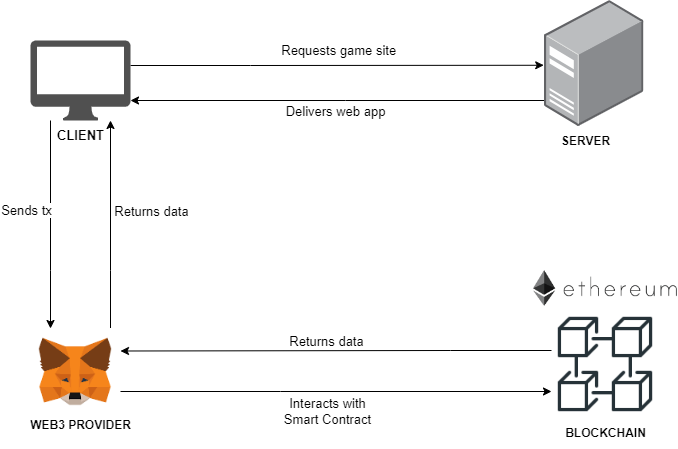
\includegraphics[scale=0.5]{images/arch.png}

\begin{figure}[htp]
    \centering
    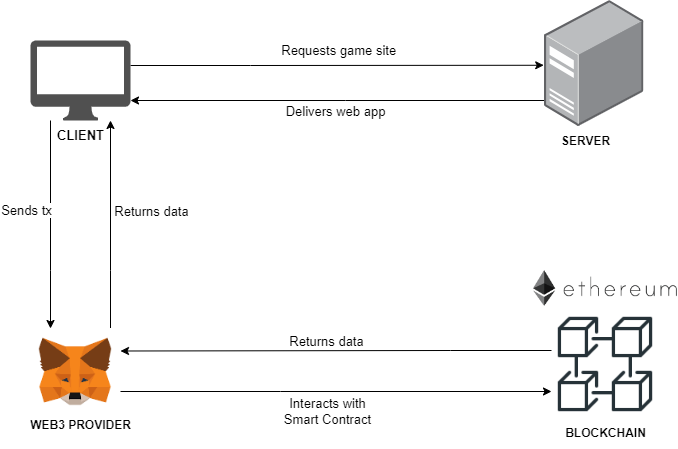
\includegraphics[scale=0.5]{images/arch.png}
    \caption{Architecture diagram}
    % \label{fig:galaxy}
\end{figure}

The client accesses the game website by entering the url in their browser with the Metamask extension. 
After which they play the game by using our frontend and sending transactions via Metamask, which interacts with the Ethereum blockchain, and hence our smart contracts deployed on it.

\paragraph{Key Components}
\begin{itemize}
\item[] \textbf{Ethereum}: It is a decentralized, open-source blockchain with smart contract functionality. Ether is the native cryptocurrency of the platform.
\item[] \textbf{Smart Contract}: They are the building blocks we use to create blockchain applications. They are programs that we can write with source code and deploy to the blockchain. They are written in the Solidity programming language. 
\item[] \textbf{MetaMask}: It serves as a web3 provider and a crypto wallet, whose purpose is to interact with the blockchain. It is distributed as a browser extension. 
\item[] \textbf{Ethers js}: It is a popular library that encodes and decodes any data prior to, or after interaction with the blockchain.

\end{itemize}



\section{Implementation}

\subsection{Game features}

\begin{itemize}
    \item[] \textbf{Judge}:
    There is a predecided judge who is responsible for approving (validating) each
    submitted word in the game.
    \item[] \textbf{Validation Condition}:
    Apart from the condition mentioned in the problem, a word is deemed valid by the
    judge if it has not been used previously (thus we do not allow repitition of words)
    and also if it comes from the dictionary implemented in \verb|worddict.js|.
    \item[] \textbf{Lives}:
    We have implemented a system of lives. All new players get 3 lives. A life is lost upon submission of an invalid word. Losing all lives results in elimination. When a player passes a turn, they lose a life. 
    \item[] \textbf{Terminating/winning condition}: 
    Our terminating condition is through \textbf{last man standing}. When all but one
    player have been eliminated through the process described above, the remaining
    player is declared the winner.
    
\end{itemize}

\subsection{Development tools} 

\subsubsection{Truffle}

\href{https://trufflesuite.com/}{\textit{The Truffle Suite}}:
Truffle advertises itself as ``the most comprehensive suite of tools for smart
contract development". 
\paragraph{How it can be used}:
Truffle can be used as a development environment, testing framework, and asset
pipeline for blockchains using the \emph{Ethereum Virtual Machine} (\textbf{EVM}).
It manages the entire workflow efficiently for any blockchain-based development.
Its key features include:
\begin{itemize}
    \item Built-in smart contract compilation, linking, deployment, and binary management.
    \item Deployments and transactions through MetaMask to protect our mnemonic.
    \item External script runner that executes scripts within a Truffle environment.
\end{itemize}
\paragraph{How we use it}:
Our backend is Truffle-based. We have used it for testing our software without having to use the actual Ethereum blockchain and spending actual gas on it.

\href{https://trufflesuite.com/ganache/}{\textit{Ganache}}:
Ganache is a tool for producing "One-click blockchains". It is a personal blockchain for developing software for Ethereum or even Corda. 
\paragraph{How it can be used}:
Using Ganache enables:
\begin{itemize}
    \item \verb|console.log| in Solidity
    \item Forking any Ethereum network without waiting to sync
    \item Ethereum JSON/RPC support
    \item Impersonating any account without requiring any actual private keys
    \item Listening for JSON-RPC 2.0 requests over HTTPS/WebSockets
    \item Mining blocks instantly, on-demand, or at an interval.
\end{itemize}
among other things.

\paragraph{How we use it}:
Ganache has also been used for testing, by simulating players using fake private keys and addresses and observing how our code interacts with requests and events.

\subsubsection{User Interface tools} 
    \paragraph{Svelte}: It is a front-end, open-source JavaScript framework  for building UI components for web applications, similar to React, Angular, or Vue. However, unlike the others which ship a runtime component such as Virtual DOM to the browser in order to make the code run, Svelte is a compiler. It converts the declarative code written by the programmer to imperative code that works with native browser APIs. As a result, it provides highly performant code in a small package.

    \paragraph{Tailwind}: It is a collection of tiny CSS utility classes for quickly and consistently building good-looking websites. Adam Wathan, the creator of Tailwind, maintains that "semantic class names are the reason CSS is hard to maintain", i.e., it is nigh impossible to name CSS classes in a sane way and that is what makes CSS so challenging. Unlike frameworks such as Bootstrap and Material, which address this challenge by creating styles for high-level components such as buttons, dropdowns and forms, Tailwind takes a more \textbf{functional} approach by providing utility classes that can be composed together in various ways to build components.

\subsection{Backend}

\subsubsection{Events}
Events are essentially a way to write to the Ethereum logs. These logs send out notifications when new entries are made and have been set up in a way that you can subscribe or watch for new entries.
We listen to these events to update the frontend.

\paragraph{Defining events}:
\begin{lstlisting}[language=Solidity]
      ...
      event NewPlayer(address player);
      event PlayerDead(address player);
      event GameStart(address cont);
      event Approval(string word);
      event Turn(address player, uint256 turn, string word, bool correct);
      ...
\end{lstlisting}

\paragraph{Emitting events}:
  \begin{lstlisting}[language=Solidity]
    ...
    function startGame() public returns (bool) {
    if (started || msg.sender != owner) return false;
    started = true;
    emit GameStart(address(this));
    return true;
    }
    ...
\end{lstlisting}







\subsubsection{Code}

\dirtree{%
.1 truffle.
.2 contracts.
.3 WordGame.sol.
.3 WordGameFactory.sol.
.2 migrations.
.3 1\_deploy\_contract.js.
.2 test.
.3 wordgame\_test.js.
.3 wordgamefactory\_test.js.
.2 truffle-config.js.
% % .3 \hyperref[dir1-file1]{''file1''}.
}

\paragraph{Files}

\begin{itemize}
    \item \verb|WordGame.sol| : This source file contains the word-game contract which contains the functions that implement the game 
    \item \verb|WordGameFactory.sol| : This creates a \textbf{factory contract} for the Word Game contract class. A factory contract is used to deploy new smart contracts from a smart contract class
    \item \verb|1_deploy_contract.js| : This deploys the factory contract
    \item \verb|wordgame_test.js| : This file contains test cases for the \verb|WordGame.sol| contract
    \item \verb|wordgamefactory_test.js| : This file contains test cases for the \verb|WordGameFactory.sol| contract
    \item \verb|truffle-config.js| : This is the Truffle configuration file
\end{itemize}


% \newpage

\subsection{Frontend}

The frontend allows the user to create games, join existing games, and look at words already played. 
% Have an image of the UI 




\subsubsection{Code}

\dirtree{%
.1 client.
.2 src.
.3 lib.
.4 Game.svelte.
.4 GameScreen.svelte.
.4 MetaMask.svelte.
.4 Navbar.svelte.
.4 PlayersTab.svelte.
.4 CreateJoin.svelte.
.4 WaitingScreen.svelte.
.4 WordsTab.svelte.
.3 App.svelte.
.2 scripts.
.3 judge.js.
.3 worddict.json.
}

\paragraph{Files}

\begin{itemize}
    \item \verb|Game.svelte| :  Combines and displays either the Gamescreen or the Start/Join screen or the Waiting screen depending on the stage  
    \item \verb|GameScreen.svelte| : Contains the HTML UI elements of the game screen, like text field to enter the word, button to submit the word, etc, and the code for events related to these elements. 
    \item \verb|MetaMask.svelte| : Checks if the user has installed the MetaMask plugin and connects to the user's MetaMask account
    \item \verb|Navbar.svelte| : Contains UI elements for the navigation bar
    \item \verb|PlayersTab.svelte| : Shows the list of players who currently joined the game.
    \item \verb|CreateJoin.svelte| : Contains buttons to Start and Join the game, and their functionality. 
    \item \verb|WaitingScreen.svelte| : Displays the waiting screen which is the screen shown after we have joined a game but the game has not started yet
    \item \verb|WordsTab.svelte| : Contains and displays a list of the last five/six
    words submitted
    \item \verb|judge.js| : Waits for an approval event from WordGame contract and sets the approval to be true if the word is in the dictionary \verb|worddict.json|
    \item \verb|worddict.json| : This is a dictionary of valid words
\end{itemize}


\section {Challenges/Improvements}
It was not possible to include a timer because you have to keep track of transaction hash rate: essentially the only way to know time is when a new block is added to the blockchain. For an auction, this is fine since any transaction after the time limit can be discarded. However, for our game, we want to ensure that every player has a time limit after which the turn proceeds to the next player and every player needs to know which player failed to answer within the time limit. 

It was also not possible to include a Merkle tree due to lack of time which would have gotten rid of the judge. Instead, we have used a JS script \verb|judge.js|. It is itself outside the blockchain but is connected to the blockchain via an account. It listens for an approval event from the game contract and sends approval accordingly.

\end{document}